\documentclass[12pt, russian, a4paper]{article}

% packages

\usepackage[a4paper, includefoot,
            left=2.5cm, right=1.5cm,
            top=1.5cm, bottom=1.5cm,
            headsep=1cm, footskip=1cm]{geometry}

\usepackage[utf8]{inputenc}
\usepackage[T2A]{fontenc}
\usepackage[english, main=russian]{babel}
\usepackage{graphicx}
\usepackage{amssymb}
\usepackage{amsfonts}
\usepackage{amsmath}
\usepackage{amsthm}
\usepackage{physics}
\usepackage{nicefrac}
\usepackage{cancel}
\usepackage{hyperref}
\usepackage{cmap}
%\usepackage{tempora}
\usepackage{indentfirst}
\usepackage{multirow}

\usepackage{caption}
\usepackage{subcaption}

\newcommand{\Section}[1]{\clearpage % put new chapters on a new page
\refstepcounter{section} % manually increment the chapter number
% manually add the chapter to the table of contents
\addcontentsline{toc}{section}{\protect\numberline{\thesection.}#1}
% and now format the header according to spec.
\begin{center}
\textbf{\protect{\thesection.}\ \ #1}
\end{center}
}

\newcommand{\Anonsection}[1]{\clearpage % put new chapters on a new page
\addcontentsline{toc}{section}{#1}
% and now format the header according to spec.
\begin{center}
\textbf{\protect{#1}}
\end{center}
}

\newcommand{\Subsection}[1]{% put new chapters on a new page
\refstepcounter{subsection} % manually increment the chapter number
% manually add the chapter to the table of contents
\addcontentsline{toc}{subsection}{\protect\numberline{\thesubsection.}#1}
% and now format the header according to spec.
\begin{center}
\textbf{\protect{\thesubsection.}\ \ #1}
\end{center}
}

\usepackage{setspace}
\onehalfspacing % Полуторный межстрочный интервал
\parindent 1.27cm % Абзацный отступ

\addto{\captionsrussian}{\renewcommand*{\contentsname}{\normalsize\centering СОДЕРЖАНИЕ}}

\addto{\captionsrussian}{\renewcommand*{\refname}{\normalsize\centering СПИСОК ЛИТЕРАТУРЫ}}

\begin{document}
	%!TEX root = ../diode.tex
\begin{titlepage}
	\begin{center}
	% \vspace{-3em}
	{\textsc{Нижегородский государственный университет имени Н.\,И. Лобачевского}}
	\vskip 2pt \hrule \vskip 3pt
	{\textsc{Высшая школа общей и прикладной физики}}

	\vfill


	{{\large Отчет по лабораторной работе}\vskip 12 pt {\Large \bfseries НАБЛЮДЕНИЕ СПЕКТРА ИЗЛУЧЕНИЯ ГЕЛИЙ-НЕОНОВОГО ЛАЗЕРА ПРИ ПОМОЩИ ТРЕХЗЕРКАЛЬНОГО КОЛЬЦЕВОГО РЕЗОНАТОРА}}

		
	\vspace{2cm}
	{\large Работу выполнили студенты \\[0.5em]{\Large \bfseries Поляков Андрей, Козлов Александр, Роганов Николай, Былинский Никита}}

	\end{center}

	\vfill

	\begin{center}
	{Нижний Новгород, \today}
	\end{center}
\end{titlepage}
	\setcounter{page}{2}

	\Section{ТЕОРИЯ}

	\Subsection{ЧАСТОТНЫЕ ХАРАКТЕРИСТИКИ ГАЗОВОГО HE-NE ЛАЗЕРА}

	В He-Ne лазере в качестве активной усиливающей свет среды используется смесь инертных газов гелия и неона при низком давлении (единицы миллиметров ртутного столба), которая возбуждается тлеющим разрядом. Инверсия населенности уровней создается в нейтральных атомах неона, а гелий играет вспомогательную роль «резервуара» для создания избыточно энергии, полученной при столкновении с электронами. Гелий в процессе неупругих столкновений с неоном передает ему энергию, населяя верхний рабочий уровень. Нижним возбужденным состояниям атома гелия $2^1s_0$ и $2^3s_1$ соответствуют избыточная внутренняя энергия 20,61 и 19,82 эВ соответственно.

	He-Ne лазер может работать в двух режимах генерации: в режиме  генерации на нескольких продольных модах резонатора и в режиме одночастотной генерации. В первом случае спектр состоит из чрезвычайно узких спектральных линий, во втором случае --- из одной спектральной линии. Как следует из рисунка \ref{fig:he-ne-enrgy} генерация на волне 632.8 нм обеспечивается переходом $3s_2\rightarrow2p_4$ в атоме Ne, генерация на волне 1153 нм --- переходом $2s_2\rightarrow2p_4$, а генерация на волне 3309 нм --- переходом $3s_2\rightarrow3p_4$.

	\begin{figure}[htbp]
		\centering
		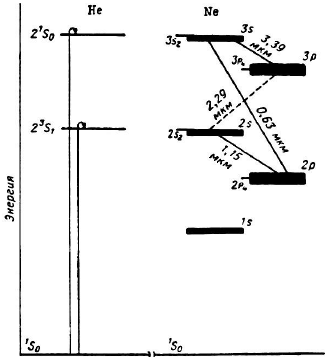
\includegraphics[scale=0.8]{he-ne-enrgy.png}
		\caption{Диаграмма нижних энергетических состояний гелия и неона.}
		\label{fig:he-ne-enrgy}
	\end{figure}

	Переходы $3s_2\rightarrow2p_4$, $2s_2\rightarrow2p_4$ и $3s_2\rightarrow3p_4$ имеют различный характер уширения. Характер уширения однородный или не однородный, когда в процессе генерации на одной частоте участвуют, соответственно, все, или часть компонент спектральной линии, определяется соотношением трех процессов. Это естественное, столкновительное и доплеровское уширения. В He-Ne лазере при генерации на переходе $3s_2\rightarrow2p_4$ ($\lambda = 632.8\,\textnormal{нм}$) и на переходе $2s_2\rightarrow2p_4$ ($\lambda = 1153\,\textnormal{нм}$) уширение спектральной линии имеет неоднородный характер, в то время как при генерации $3s_2\rightarrow3p_4$ ($\lambda = 3309\,\textnormal{нм}$).

	Рассмотрим основные особенности спектра излучения, формируемого при помощи резонатора Фабри-Перо в пределах части спектральной линии спонтанного излучения, в которой усиление света превышает уровень потерь. Под \emph{полной шириной полосы резонатора на полувысоте} понимают
	\begin{equation}
		\Delta \nu_c = \dfrac{cf}{2\pi L},\quad f = \mathrm{ln}\qty(\dfrac{1}{\sqrt{R_1R_2}}),
	\end{equation}
	где $c$ --- скорость света в вакууме, $R_{1,2}$ --- коэффициенты отражения зеркал, $f$ --- потери за один обход. Величина $c/2L$ определяет частотный интервал между основными типами колебаний интерферометра Фабри-Перо. Заметим, что для $f=0.009$ и $L=0.4\,\textnormal{м}$ $\Delta \nu_c$ получается примерно $1\,\textnormal{МГц}$, а $c/2L$ составляет около 375 МГц.

	\emph{Однородной шириной} $\Delta \nu_a$ перехода $3s_2\rightarrow2p_4$ ($\lambda = 632.8\,\textnormal{нм}$) изолированного атома Ne является \emph{естественная ширина} линии $\Delta \nu_n$, которая определяется конечностью времени жизни верхнего и нижнего уровней энергии перехода и составляет около 20 МГц.

	Оптимальное давление газовой смеси He-Ne для генерации на волне 632.8 нм, настолько низко, что доплеровское уширение линии спонтанного излучения многократно превышает уширение из-за столкновений. \emph{Доплеровский сдвиг} можно оценить следующим образом:
	\begin{equation}
		\Delta \nu_D = 7\times10^{-7}\,\nu_0\,\sqrt{\dfrac{T \textnormal{ [К]}}{M}},
	\end{equation}
	где $M=20$ – молекулярная масса, $T \textnormal{ [К]}$ – температура в Кельвинах, $\nu_0$ - частота перехода. При $T=400\,\textnormal{К}$ величина доплеровского сдвига на волне 632 нм составляет $\sim$1500 МГц. Таким образом, линия спонтанного излучения многократно уширена относительно естественной ширины линии перехода и приблизительно равна 1500 МГц. Поэтому переход $3s_2\rightarrow2p_4$ ($\lambda = 632.8\,\textnormal{нм}$) является \emph{неоднородно уширенным}, то есть в пределах данного перехода возможно возбуждение нескольких частот резонатора Фабри-Перо.

	Итог такому рассмотрению спектральных характеристик можно заключить с помощью следующего неравенства:
	\begin{equation}
		\Delta \nu_c < \Delta \nu_n = \Delta \nu_a < c/2L < \Delta \nu_D.
	\end{equation}

 
\end{document}